\chapter[Gestão de projeto]{Gestão de projeto}

\section{Recursos Humanos}

Para uma melhor organização do grupo e distribuição de atividades e responsabilidades, foi criada uma hierarquia de responsabilidades na equipe do projeto, elegendo um líder para representar o grupo e gerenciar o projeto e um sub-líder para cada engenharia, com exceção das engenharias automotiva e aeroespacial que estão trabalho na mesma área. Cada sub-líder é responsável por gerenciar as atividades de cada engenharia e facilitar a comunicação com as outras engenharias. É importante frisar que essa divisão é apenas uma forma de organizar a equipe, facilitando a divisão de atividades e responsabilidades de cada área da engenharia, mas no decorrer do projeto todas as engenharias terão que trabalhar de forma integrada.

\begin{figure} [!htp]
	\centering
	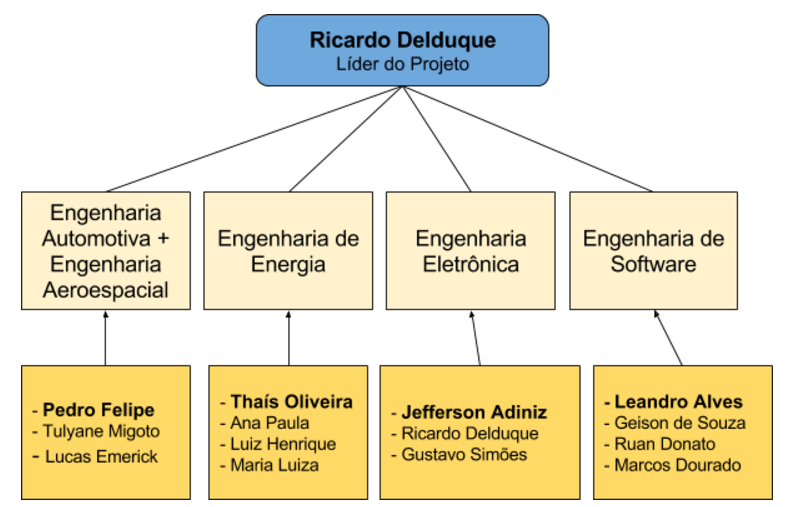
\includegraphics[scale=0.55]{figuras/rh.png}
	\caption{Organograma de hierarquia de Recursos Humanos}
	\label{EAP}
\end{figure}

\begin{itemize}
    \item Líder do Projeto: representante do grupo em geral, responsável por gerenciar o andamento do projeto, distribuir tarefas, cobrar resultados, marcar reuniões e etc.
    
    \item Engenharia Automotiva e Engenharia Aeroespacial: responsável por toda estrutura do barco
    
    \item Engenharia de Energia: responsável pelas fontes energéticas inerentes ao projeto
    
    \item Engenharia de software: responsável pela elaboração, construção e implantação da solução de software do projeto.
    
    \item Engenharia Eletrônica: responsável pela elaboração e implementação da parte eletrônica do projeto.
\end{itemize}

\section{Acompanhamento do projeto}

Para o planejamento e acompanhamento do projeto optou-se por dividir o projeto em fases: Iniciação, Planejamento, Execução e Encerramento. Para cada uma destas fases foram definidas os itens planejados para a conclusão do projeto. Para o Ponto de Controle 1 foram executadas as fases de Iniciação e Planejamento. Para o Ponto de Controle 2 será realizada a fase de Execução. Na fase de Encerramento será realizado a integração, obtendo o produto final e a apresentação do mesmo no Ponto de Controle 3.


 \begin{figure} [!htp]
	\centering
	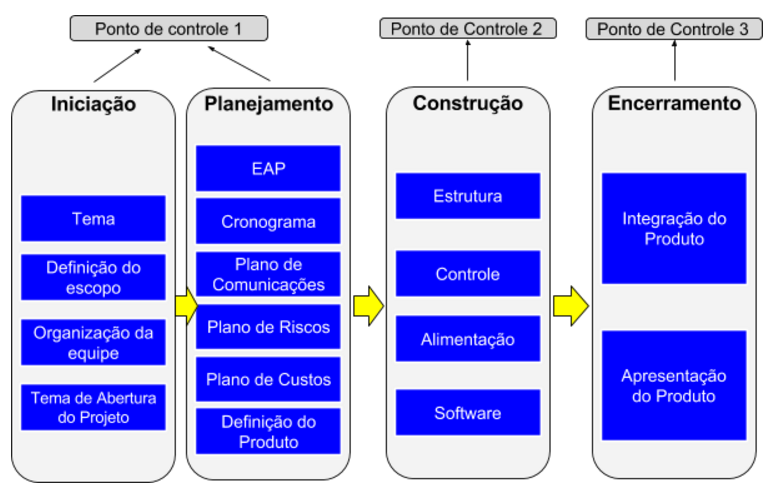
\includegraphics[scale=0.55]{figuras/fases}
	\caption{Fases do projeto}
	\label{EAP}
\end{figure}


\section{Estrutura Analítica do projeto(EAP)}

Para um melhor controle da evolução do projeto e correções mais pontuais, a EAP deste projeto será elaborada em grupos de entregas, componentes menores e mais gerenciáveis. Possibilitando a melhor alocação dos recursos e determinação de pontos que exigirão força tarefa.

 \begin{figure} [!htp]
	\centering
	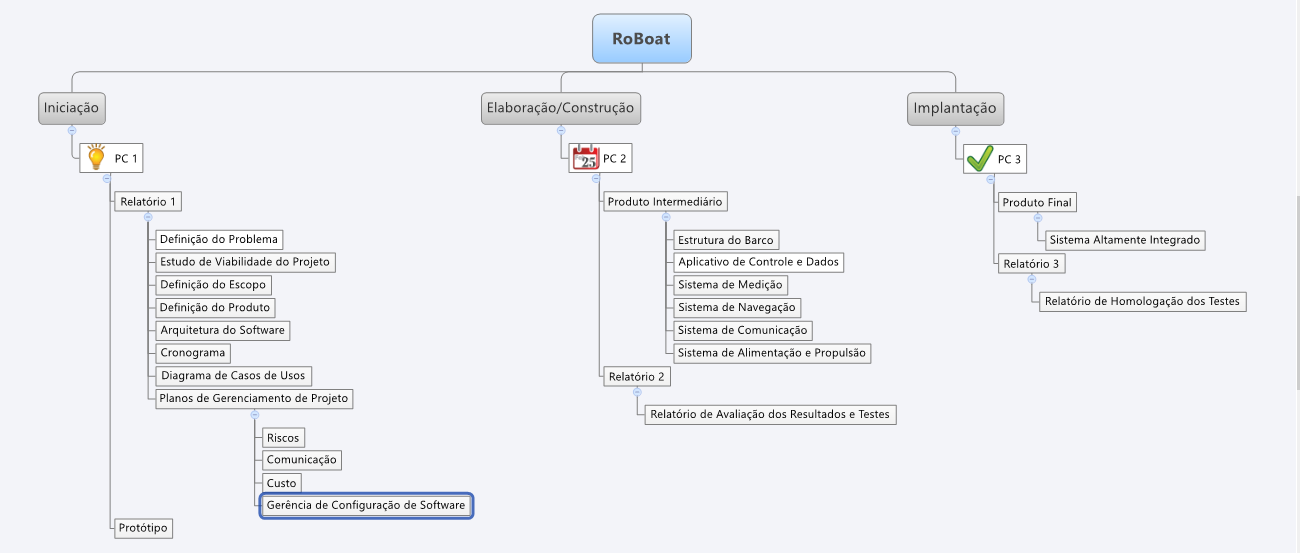
\includegraphics[scale=0.5]{figuras/EAPPI}
	\caption{Estrutura analítica do projeto.}
	\label{EAP}
\end{figure}


\section{Cronograma}

Cronograma inicial para auxiliar no controle das atividades e gerenciamento, neste cronograma estão descritas as fases, atividades e entregas do projeto e suas respectivas datas de início e término.
\FloatBarrier
\begin{table}[]
\centering
\caption{Cronograma}
\label{tab:cronograma}
\begin{tabular}{|l|l|l|}
\hline
\textbf{Fase/Atividade} & \textbf{início} & \textbf{fim} \\ \hline
\multicolumn{3}{|c|}{Fase de Iniciação} \\ \hline
Definição do tema e grupo & 08/03/2017 & 15/03/2017 \\ \hline
Definição do escopo & 15/03/2017 & 17/03/2017 \\ \hline
Termo de Abertura do Projeto & 17/03/2017 & 22/03/2017 \\ \hline
\multicolumn{3}{|c|}{Fase de Planejamento} \\ \hline
Elaboração da EAP & 22/03/2017 & 24/03/2017 \\ \hline
Elaboração do cronograma & 24/03/2017 & 29/03/2017 \\ \hline
Elaboração do plano de comunicação & 22/03/2017 & 29/03/2017 \\ \hline
Elaboração do plano de riscos & 22/03/2017 & 29/03/2017 \\ \hline
Elaboração do plano de custos & 22/03/2017 & 29/03/2017 \\ \hline
Descrição do produto & 22/03/2017 & 29/03/2017 \\ \hline
Elaboração do organograma & 22/03/2017 & 29/03/2017 \\ \hline
Elaboração do cronograma & 22/03/2017 & 29/03/2017 \\ \hline
Diagrama de casos de uso & 22/03/2017 & 29/03/2017 \\ \hline
Definição da arquitetura do software & 22/03/2017 & 29/03/2017 \\ \hline
Elaboração do relatório do ponto de controle 1 & 22/03/2017 & 29/03/2017 \\ \hline
Revisão do relatório ponto de controle 1 & 29/03/2017 & 31/03/2017 \\ \hline
Entrega relatório ponto de controle 1 & 31/03/2017 & 31/03/2017 \\ \hline
Apresentação do ponto de controle 1 & 05/04/2017 & 07/04/2017 \\ \hline
\multicolumn{3}{|c|}{Fase de Execução} \\ \hline
Simulação Catia /Ansys & 01/04/2017 & 10/04/2017 \\ \hline
Aquisição dos materiais & 01/04/2017 & 10/04/2017 \\ \hline
Manufaturação & 11/04/2017 & 20/05/2017 \\ \hline
Desenvolver a pá & 01/04/2017 & 05/05/2017 \\ \hline
Aquisição dos materiais & 30/03/2017 & 28/04/2017 \\ \hline
Montar o sistema & 06/05/2017 & 19/05/2017  \\ \hline
Aquisição dos materiais & 30/03/2017 & 14/04/2017 \\ \hline
Fabricação dos sensores & 30/03/2017 & 20/04/2017 \\ \hline
Calibrar sensores & 17/04/2017 & 28/04/2017 \\ \hline
Comunicação entre RoBoat e Base & 14/04/2017 & 28/04/2017 \\ \hline
Armazenar dados SD & 01/04/2017 & 05/05/2017 \\ \hline
Monitoramento via GPS & 14/04 & 28/04/2017 \\ \hline
Aplicação Desktop &  17/04/2017 & 09/05/2017 \\ \hline
Revisão do relatório ponto de controle 2 & 24/05/2017 & 25/05/2017 \\ \hline
Entrega relatório ponto de controle 2 & 26/05/2017 & 26/05/2017 \\ \hline
Apresentação ponto de controle 2 & 31/05/2017 & 02/06/2017 \\ \hline
\multicolumn{3}{|c|}{Fase de Encerramento} \\ \hline
Integração & 03/06/2017 & 04/07/2017 \\ \hline
Revisão do relatório ponto de controle 3 & 28/06/2017 & 29/06/2017 \\ \hline
Entrega relatório ponto de controle 3 & 30/06/2017 & 30/06/2017 \\ \hline
Apresentação do Produto & 05/07/2017 & - \\ \hline
\end{tabular}
\end{table}
\FloatBarrier
\section{Termo de Abertura do Projeto}

Plano de Abertura do Projeto:

\subsection{Introdução e Justificativa}

O RoBoat é uma embarcação inteligente controlada remotamente. Sua função é auxiliar na coleta e análise de água em pontos estratégicos de lagos, rios e reservatórios. A idéia do projeto surgiu da necessidade de se medir de forma autônoma, e obter dados em tempo real, sobre a qualidade da água em locais onde a logística demanda demasiadamente recursos financeiros e tempo. Dessa forma empresas poderiam utilizar recursos humanos menos especializados, poupar tempo e obter dados em intervalos de tempo menor. Além de evitar desastres ecológicos, evitarão possíveis multas e possíveis perdas de maquinário por corrosão entre outros danos causados pelo contato da água.
      
\subsection{Visão Geral do Produto}

Para ter uma visão clara foi usado o mapeamento de atividade no modelo 5W2H:

\textbf{What}: Barco a motor controlado que coleta e disponibiliza em tempo real informações sobre a água do local;

\textbf{Why}: O intuito é que se conheça a qualidade da água, para posteriormente, planeje-se ações;

\textbf{Where}: Lagos, rios e reservatórios;
Who: Alunos do curso de Engenharia de Software, Energia, Automotiva, Aeroespacial e Eletrônica da Universidade de Brasília.

\textbf{When}: Parte do projeto será realizado no período de um semestre, ou seja, 15 semanas.

\textbf{How}: O PMBOK será a referência principal em relação a gerência de projetos. Sendo que esse projeto será desenvolvido em três entregas.

\section{PLano de Gerenciamento de Configuração de Software}


Este plano tem como objetivo descrever as tecnologias e ferramentas utilizadas para o desenvolvimento da solução de software do projeto, como também definir os métodos adotados para o controle de configuração de software.

A intenção do gerenciamento de configuração é estabelecer e manter a integridade da solução de software do projeto durante seu ciclo de vida.  Esse plano contém todas as informações referentes ao sistema de gerenciamento de configuração para o projeto. As ferramentas utilizadas foram previamente definidas, como também suas respectivas versões, afim de manter a padronização entre a equipe e evitar problemas de ambiente durante o desenvolvimento.

\textbf{Ferramentas e tecnologias}

\begin{itemize}
    \item \textbf{GIT}: Sistema de controle versão: usado para versionamento do código.
    \item \textbf{Github}: Servidor para armazenamento do código fonte.
    \item \textbf{Linguaguem}: Ruby. Versão 2.3.xx
    \item \textit{\textbf{Frameworks}}:
    \begin{itemize}
        \item \textbf{Artoo}: Framework de controle de arduíno
        \item \textbf{ruby-xbee}: \textit{Gem} para ruby para comunicação com Xbee. Versão: 1.2.0
        \item \textbf{Firmata}: Protocolo de comunicação com arduino. Versão: 0.4.6
    \end{itemize}
\end{itemize}

O repositório está dividido em duas branches principais, Master e Development, e diversas branches auxiliares, Features.

\begin{itemize}
\item \textbf{Master}: Branch que conterá as versões estáveis e os lançamentos do projeto.
\item \textbf{Development}:  Branch utilizada para controle de entregas, cada iteração/sprint será desenvolvida dentro desta branch.
\item \textbf{Feature}: Para cada Caso de Uso deverá ser criada uma nova branch, de forma que se torne possível trabalhar em áreas diferentes da aplicação de forma organizada.
\end{itemize}
